% Chapter X

\chapter{Introduction and Background} % Chapter title

\label{ch:intro} % For referencing the chapter elsewhere, use \autoref{ch:name} 

The very first step in development of a numerical simulation for a one way quantum computer, is to define terms so that the accuracy of the model can be checked. To this aim, we first establish a definition of cluster states as well as the features of a measurement based quantum computer so that we can examine the functionality of the one way quantum computer.

%----------------------------------------------------------------------------------------


\section{Cluster States}

The main phenomenon enabling measurement based quantum computation is through the use of cluster states \citep{briegel_measurement-based_2009}. These states are formed of N qubits interacting with each other in arrays with a high 'persistency' of entanglement \citep{briegel_persistent_2000}. Persistency is defined in 'Persistent entanglement in arrays of interacting particles' as the minimum number of local measurements such that the state is completely disentangled for all measurement outcomes. This property means that measurements can be made on individual qubits in the state that will not entirely disentangle the state \citep{briegel_persistent_2000}, allowing information to be passed from one qubit to another. Additionally, the states are also said to be 'maximally connected' if they measurements on qubits in a set can project two seperate qubits into a pure Bell state \citep{briegel_persistent_2000}. This has the advantage of allowing easily teleportable states be produced through measurements on these cluster states.

These states are generally formed in either optical lattices \citep{joo_generating_2012} or from photons \citep{kiesel_experimental_2005, walther_experimental_2005}, though other implementations are possible \citep{briegel_measurement-based_2009}.

%----------------------------------------------------------------------------------------

\section{Measurement Based Quantum Computation}

The term 'measurement based quantum computer' refers to a whole class of quantum computer architectures that use measurements instead of unitary operators to process information \citep{jozsa_introduction_2005}. Unlike some other 'alternative' methods of quantum computation, such as quantum annealing devices, Measurement based quantum computers are both universal and do not suffer from as greatly from problems with decoherence as qubits are discarded after measurement \citep{jozsa_introduction_2005}. However, different challenges arise from the difficulty in forming the required states and then measuring specific qubits \citep{briegel_measurement-based_2009}. 

In the specific case of the one way quantum computer, using the two properties of cluster states mentioned earlier, it is possible to perform measurements on a 'lattice' of entangled particles in order to form a kind of quantum circuit that processes information \cite{raussendorf_one-way_2001} and this is illustrated in figure \ref{fig:one_way}. The exact functionality of these circuits will be shown in the next section.

\begin{figure}
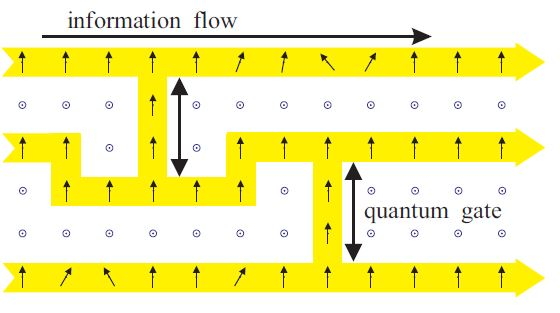
\includegraphics[scale=0.7]{gfx/infoflow.JPG}
\caption{Sketch of information flow in one way computation \citep{raussendorf_measurement-based_2003}}
\label{fig:one_way}
\end{figure}

